\PassOptionsToPackage{svgnames}{xcolor}
\documentclass[11pt]{article}



\usepackage[margin=0.1in]{geometry}  
\usepackage{graphicx}             
\usepackage{amsmath}              
\usepackage{amsfonts}              
\usepackage{framed}               
\usepackage{amssymb}
\usepackage{array}
\usepackage{amsthm}
\usepackage[nottoc]{tocbibind}
\usepackage{bm}
\usepackage{enumitem}


  \newcommand\norm[1]{\left\lVert#1\right\rVert}
\setlength{\parindent}{0cm}
\setlength{\parskip}{0em}
\newcommand{\Lim}[1]{\raisebox{0.5ex}{\scalebox{0.8}{$\displaystyle \lim_{#1}\;$}}}
\newtheorem{definition}{Definition}[section]
\newtheorem{theorem}{Theorem}[section]
\newtheorem{notation}{Notation}[section]
\theoremstyle{definition}
\DeclareMathOperator{\arcsec}{arcsec}
\DeclareMathOperator{\arccot}{arccot}
\DeclareMathOperator{\arccsc}{arccsc}
\DeclareMathOperator{\PV}{PV}
\DeclareMathOperator{\TV}{TV}
\DeclareMathOperator{\diff}{d}
\DeclareMathOperator{\expec}{E}
\DeclareMathOperator{\var}{Var}
\DeclareMathOperator{\cov}{Cov}
\DeclareMathOperator{\CE}{CE}
\DeclareMathOperator{\RP}{RP}
\newcommand\cf[1]{\mathbf{#1}}
\setcounter{tocdepth}{1}
\begin{document}
\twocolumn
\section{Preliminary Result}
\subsection{Newton Rhapson Method}
\[
x_{i+1} = x_i-\frac{f(x_i)}{f^\prime(x_i)}
\]
\subsection{A result from Tutorial 6}
Given an initial wealth of $w_0$ and two investments $X_1$ and $X_2$ with rates of returns $r_1$ and $r_2$ respectively, where $r_i\sim N(\mu_i, \sigma_i^2)$, a risk averse investor whose utility function is any positive affine transformation of $U(x)=-e^{-\lambda x}, \lambda>0$ allocates $\alpha W_0$ in $X_1$ and $(1-\alpha)W_0$ in $X_2$ where $\alpha\in[0,1]$ in such a way that
\[
f(\alpha) = \alpha(\mu_1)+(1-\alpha)\mu_2-\frac{\lambda W_0}{2}(\alpha^2\sigma_1^2+(1-\alpha)^2\sigma_2^2)
\]
\section{Expected Utility Theory}
\subsection{Expected Utility and Risk Attitude}
\begin{definition}[Expected Utility]
\hfill\\\normalfont An individual with an initial wealth of $w_0$ is considering a \textbf{risky prospect}with a random payoff $X$. He is assumed to have a \textbf{utility function} that is real-valued, continuous and \textbf{increasing}. He will make his investment decision based on the \textbf{expected utility} of his final wealth $W:=X+w_0$, defined as follows.
\begin{itemize}
  \item \textbf{Discrete $X$}\\If the risky investment has $n$ possible mutually exclusive payoffs $(x_1,x_2,\ldots, x_n)$ with associated probabilities $p_1,p_2,\ldots, p_n)$, where $\sum_{i=1}^n p_i = 1$, then the \textbf{expected utility} of the individual's final wealth $W$, is given by
  \[
\expec[ U (W)]=\expec[ U (X+w_0)] := \sum_{i=1}^n p_i U (x_i+w_0)
  \]
\item If $X$ is a continuous random variable having a density function $f:(a,b)\to(0,\infty)$, then
\[
\expec[ U (X+w_0)]:=\int_a^b f(x) U (x+w_0)\diff x
\]
\end{itemize}
\end{definition}
\begin{definition}[Utility-based Decision]\hfill\\\normalfont
Under \textbf{utility-based decision}, he individual will
\begin{itemize}
  \item \makebox[4.5cm][l]{invest in the risky prospect}\makebox[1cm]{if}$\expec[ U (X+w_0)]> U (w_0)$.
  \item \makebox[4.5cm][l]{avoid the risky prospect}\makebox[1cm]{if}$\expec[ U (X+w_0)]< U (w_0)$.
    \item \makebox[4.5cm][l]{be indifferent }\makebox[1cm]{if}$\expec[ U (X+w_0)]= U (w_0)$.
  \end{itemize}
  \end{definition}
Given a set of risky prospects, an individual will \textit{most} favour the one that maximises the expected utility of his final wealth.
\begin{definition}[Characterisation of Risk Attitude]\hfill\\\normalfont
An individual with utility function $U$ is said to be
\begin{itemize}
  \item \makebox[3cm][l]{risk averse}\makebox[1cm]{if}$U$ is strictly concave.\footnote{A function $U$ is strictly concave on $I$ if $U^{\prime\prime}<0$ on $I$.}
  \item \makebox[3cm][l]{risk neutral}\makebox[1cm]{if}$U$ is linear.
  \item \makebox[3cm][l]{risk loving}\makebox[1cm]{if}$U$ is strictly convex.
\end{itemize}
\end{definition}
By Jensen Inequality, we deduce
\begin{theorem}[Equivalent condition for Risk Attitude Characterisation]
\hfill\\\normalfont 
\begin{itemize}
  \item \makebox[3cm][l]{risk averse}\makebox[1cm]{if}$\expec[ U (W)]< U [\expec(W)]$.
  \item \makebox[3cm][l]{risk neutral}\makebox[1cm]{if}$\expec[ U (W)]= U [\expec(W)]$
  \item \makebox[3cm][l]{risk loving}\makebox[1cm]{if}$\expec[ U (W)]> U [\expec(W)]$
\end{itemize}
for \textbf{any} risky investment that yields a final wealth of $W$.
\end{theorem}
\begin{definition}[Positive Affine Transformation]\hfill\\\normalfont
Let $ U $ be an utility function. For any $\alpha>0, \beta\in\mathbb{R}$, the function $\alpha U +\beta$ is a \textbf{positive affine transformation} of $ U $.
\end{definition}
Obviously, both function have the same attitude towards risks.
\subsection{Certainty Equivalent}
\begin{definition}[Certainty Equivalent]
\hfill\\\normalfont Let $U$ be the utility function of an individual. Given a risky prospect with payoff $X$ ,the \textbf{certainty equivalent} of $X$ with respect to $U$, is defined to be the real number $c = ]CE(X;U)$ for which
\[
U(c)=\expec(U(w_0+X))
\]
\end{definition}
It follows that an individual
\begin{itemize}
  \item \makebox[5.5cm][l]{invests in the risky prospect}\makebox[1cm]{if}$\CE(X;U)>w_0$
  \item \makebox[5.5cm][l]{avoids the risky prospect}\makebox[1cm]{if}$\CE(X;U)<w_0$
  \item \makebox[5.5cm][l]{is indifferent}\makebox[1cm]{if}$\CE(X;U)=w_0$
\end{itemize}
For positive affine transformation $\alpha U+\beta$ where $\alpha>0$, we have
\[
\CE(X, \alpha U+\beta) = \CE(X,U)
\]
\begin{definition}[Risk Premium]
\hfill\\\normalfont The \textbf{risk premium} of a risky prospect with respect to an utility function $U$ is the real number $r=\RP(X;U)$ for which
\[
U(w_0-r) = \expec(U(w_0+X))
\]
where $X$ is the payoff.
\end{definition}
Clearly,
\[
r=w_0-c
\]
and hence, an individual
\begin{itemize}
  \item \makebox[5.5cm][l]{invests in the risky prospect}\makebox[1cm]{if}$\RP(X;U)<0$
  \item \makebox[5.5cm][l]{avoids the risky prospect}\makebox[1cm]{if}$\RP(X;U)>0$
  \item \makebox[5.5cm][l]{is indifferent}\makebox[1cm]{if}$\RP(X;U)=0$
\end{itemize}
\subsection{Arrow-Pratt Measures of Risk Aversion}
\begin{definition}[Absolute Risk Aversion]
\hfill\\\normalfont For a \textit{risk averse} individual whose utility function is $U$, his \textbf{Arrow-Pratt absolute risk aversion Coefficient}(ARA) at wealth level $w$ is
\[
-\frac{U^{\prime\prime}(w)}{U^\prime(w)}
\]
\end{definition}
\begin{theorem}[ARA of positive affine transformation]
\hfill\\\normalfont $U_\text{ARA} = V_\text{ARA}$ if and only if $U$ and $V$ are positive affine transformation of each other.
\end{theorem}
We can say that two utility functions are \textbf{equivalent} if and only if they have the same ARA.\\
Suppose two individuals with utility functions $U$ and $V$ admits the following condition:
\[
U_\text{ARA}(w)>V_\text{ARA}(w)
\]
at \textbf{all} wealth level, $w$, we say the individual with utility function $U$ is \textbf{globally more risk averse} than the individual with utility function $V$.
\begin{theorem}
\hfill\\\normalfont More generally, an individual with utility function $U$ is \textbf{globally more risk averse} than an individual with utility function $V$ if and only if there is an increasing and strictly concave function $g$ such that
\[
U(w)=g(V(w))
\]
\end{theorem}
\subsection{Portfolio Selection}
An individual with an initial wealth of $w_0$ can invest a portion (say $\alpha w_0$, where $\alpha\in[0,1]$) of his money in a risky investment $X$ that has a random \textbf{rate of return}, $R$. The expected utility of his final wealth is
\[
\expec[U(W)]=\expec[U(w_0(1+\alpha R))]
\]
Note that $\frac{\diff^2}{\diff\alpha^2}\expec[U(W)]<0$ for any risk-averse individual, hence setting the first order derivative to 0 always yields maxima $\alpha^\ast$, although there is no guarantee that such $\alpha^\ast\in[0,1]$.
%\clearpage
\section{Mean-Variance Analysis}
In this chapter, the accumulation function is constant 1. Therefore, we do not consider time value.
\subsection{Return and Risk of Asset}
\begin{definition}[Rate of Return]
\hfill\\\normalfont Asset is a tradable financial instruments. We denote that each asset is traded over one time period, from $t=0$(initial) to $t=1$(end-of-period).\\
If $W_0$ invested in an asset at time $t=0$ is worth a \textbf{random} amount of $W_1$ at time $t=1$, then the \textbf{rate of return} of the asset, denoted by $r$, is a \textbf{random variable} given by
\[
r=\frac{W_1-W_0}{W_0} = \frac{W_1}{W_0}-1
\]
Equivalently, $W_1 = W_0(1+r)$.

The rate of return can also be defined in terms of the initial and end-of-period prices of the asset. Let $P_0$ be the price at $t=0$ and $P_1$ be the \textbf{random} price at $t=1$. Then
\[
r=\frac{P_1-P_0}{P_0} = \frac{P_1}{P_0}-1
\]
Equivalently, $P_1 = P_0(1+r)$,
\end{definition}
\begin{definition}[Risk of Asset]
\hfill\\\normalfont The standard deviation, $\sigma_i = \sqrt{\var(r_i)}$, of the rate of return of asset $i$, is a measure of the risk of asset $i$.
\[
\sigma_i = \sqrt{\var(r_i)}=\sqrt{\expec[(r_i-\expec(r_i))^2]} = \sqrt{\expec[r_i^2-\expec(r_i)^2]}
\]
\end{definition}
\begin{definition}[Correlation of Returns]
\hfill\\\normalfont A statistical measure of the association of the returns of two assets, $i$ and $j$, is the covariance $\sigma_{i,j} = \cov(r_i,r_j)$.
\begin{align*}
\sigma_{i,j} &= \cov(r_i,r_j) =\expec[(r_i-\expec(r_i))(r_j-\expec(r_j))]\\ 
&= \expec[r_ir_j]-\expec(r_i)\expec(r_j) = \expec[r_i(r_j-\expec(r_j))]
\end{align*}
A standardised measure is the correlation coefficient defined by
\[
\rho_{i,j} = \frac{\sigma_{i,j}}{\sigma_i\sigma_j}
\]
It can be shown that $|\rho_{i,j}|\leq 1$.
\end{definition}
\begin{definition}[Short Selling]
\hfill\\\normalfont Short selling of an asset refers to one borrowing a certain number of units of the asset from the lender at $t=0$ and seems them immediately to receive an amount $W_0$. At some preagreed date $t=1$, the short seller will buy the same number of units of the asset for an amount $W_1$ and return the asset to the lender.\\
The borrower will make a profit of $W_0-W_1$ which is positive if and only if the value of the asset falls.
\end{definition}
Obviously, the loss can be unlimited but the gain is bounded above by $W_0$.
\subsection{Portfolio Mean and Variance}
At time $t=0$, an individual invests in $n$ assets in such a way that a fraction $w_i$ of his investment capital is invested in asset $i$. It is possible that $w_i<0$, which means the individual short sells asset $i$. \\We call the vector $\mathbf{w} = (w_1,w_2,\ldots, w_n)^T$ the individual's \textbf{portfolio weight vector}, or simply \textbf{portfolio}. \\It is assumed that
\[
\sum_{i=1}^n w_i = 1
\] 
We will then have its final wealth $W_1 = \sum_{i=1}^n w_iW_0(1+r_i)$.\\
The rate of return $r_p$ of the portfolio is related to the rate of return of individual assets, $r_1$, by
\[
r_p = \sum_{i=1}^n w_ir_i
\]
It follows that the expected rate of return of the portfolio, or \textbf{portfolio mean}, is
\[
\mu_p = \expec(r_p) = \sum_{i=1}^n w_i\mu_i = \mathbf{w}^T\bm{\mu}
\]
where 
\[
\bm{\mu} = (\mu_1,\ldots, \mu_n)^T
\]
is the vector of expected rates of return of the assets $(r_1,\ldots, r_n)$ respectively. This vector is called \textbf{mean vector} for simplicity.\\
The variance of rate of return of portfolio $\var(r_p)$, or simply \textbf{portfolio variance}, of $\mathbf{w}$, is
\begin{align*}
\sigma_p^2 &= \var(r_p) = \cov(\sum_{i=1}^n w_ir_i,\sum_{j=1}^n w_jr_j )\\
&=\sum_{i=1}^n\sum_{j=1}^n w_iw_j\cov(r_i,r_j)\\
&=\sum_{i=1}^n\sum_{j=1}^n w_iw_j\sigma_{ij}\\
&=\mathbf{w}^T\mathbf{C}\mathbf{w}\text{ in matrix notation}
\end{align*}
where
\[
\mathbf{C} = \begin{pmatrix}
\sigma_{11}&\cdots&\sigma_{1n}\\
\vdots&\ddots&\vdots\\
\sigma_{n1}&\cdots&\sigma_{nn}\end{pmatrix}
\]
is known as the \textbf{covariance matrix} of the random vector $\mathbf{r} = (r_1,\cdots, r_n)$.
We also have, by noting $\sigma_{ii} = \var(r_i) := \sigma_i^2$ and $\sigma_{ij} = \sigma_{ji}$,
\[
\var(r_p) = \sum_{i=1}^n w_i^2 \sigma_i^2 + 2\sum_{i=1}^n\sum_{j<i}^n w_iw_j\sigma_{ij}
\]
\subsubsection{Diversification}
Let $\overline{\sigma}^2$ and $\overline{\phi}$ be the average variance and average covariance of an $n$ assets, that is
\[
\overline{\sigma}^2 = \frac{1}{n}\sum_{i=1}^n\sigma_i^2\;\;\;\text{ and }\;\;\;\overline{\phi}=\frac{1}{n(n-1)}\sum_{i=1}^n\sum_{\substack{j=1\\j\neq i}}^n
\] 
Suppose that $\overline{\sigma}^2\to\sigma^2$ and $\overline{\phi}\to\phi$ as $n\to\infty$, then for an equally weighted portfolio, we have
\[
\sigma_p^2 = \frac{1}{n^2}\sum_{i=1}^n \sigma_i^2 +\frac{1}{n^2}\sum_{i=1}^n\sum_{\substack{j=1\\j\neq i}}^n \sigma_{ij}\to\phi
\]
Therefore, there is limitation of diversification as a tool to reduce portfolio risk.\\While the asset specific risk $\overline{\sigma}^2$ can be driven to zero, the market wide risk, $\overline{\phi}$ cannot be eliminated even if one holds infinitely many assets.
\subsection{Portfolio of Two Assets}
Consider a portfolio with weight vector $\mathbf{w} = \begin{pmatrix}\alpha&1-\alpha\end{pmatrix}^t$ of two assets. The portfolio mean is
\[
\mu_p = \alpha\mu_1+(1-\alpha)\mu_2
\]
and
\begin{align*}
\sigma_p^2 &= \alpha^2\sigma_1^2 +(1-\alpha)^2\sigma_2^2+2\alpha(1-\alpha)\sigma_{12} = \alpha^2\sigma_1^2 +(1-\alpha)^2\sigma_2^2+2\alpha(1-\alpha)\rho_{12}\sigma_1\sigma_2 \\
&=(\sigma_1^2+\sigma_2^2-2\rho_{12}\sigma_1\sigma_2)\alpha^2+2\sigma_2(\rho_{12}\sigma_1-1)\alpha+\sigma_2^2\;\;\;\;\;(\#)
\end{align*}
\subsubsection{Global Minimum-variance Portfolio}
A risk averse individual seeks a portfolio with the \textit{smallest} risk. He will thus seek the optimal value of $\alpha$ that minimises $\sigma_p^2$.\\From the above equation $(\#), $, $\sigma_p^2$ admits a parabola concave upwards, and the minimum portfolio variance $\sigma_p^2$ occurs when
\[
\alpha=\alpha^\ast = \frac{\sigma_2(\sigma_2-\rho_{12}\sigma_1)}{\sigma_1^2+\sigma_2^2-2\rho_{12}\sigma_1\sigma_2}
\]
and the minimum portfolio variance is
\[
(\sigma_p^2)^\ast = \frac{\sigma_1^2\sigma_2^2(1-\rho_{12}^2)}{\sigma_1^2+\sigma_2^2-2\rho_{12}\sigma_1\sigma_2}
\]
The corresponding portfolio mean can then be determined from
\[
\mu_p^\ast = \alpha^\ast\mu_1+(1-\alpha^\ast)\mu_2
\]
We call the portfolio with minimum variance the global minimum-variance portfolio.
\subsubsection{Portfolio Graph}
\begin{definition}[Portfolio Graph]
\hfill\\\normalfont Portfolio graph is the graph of portfolio mean $\mu_p$ against portfolio risk $\sigma_p$.\end{definition}
From $\mu_p = \alpha\mu_1+(1-\alpha)\mu_2$, we have
\[
\alpha = \frac{\mu_p-\mu_2}{\mu_1-\mu_2}
\]
and by substituting the above equation to $(\#)$, we obtain an equation of the form
\[
\sigma_p^2 = A\mu_p^2+B\mu_p+C
\]
for some constants $A,B$ and $C$, with $A>0$.\footnote{This is due to the quadratic coefficient of $(\#)$ is greater than 0.}\\
This is an equation of a hyperbola. Rearranging
\[
\sigma_p^2 = A(\mu_p-\frac{B}{2A})^2+(C-\frac{B^2}{4A})
\]
Therefore, $\min\sigma_p^2 = C-\frac{B^2}{4A}$ at $\mu_p = -\frac{B}{2A}$. This corresponds to the global minimum-variance portfolio.\\The asymptotes of this graph are
\[
\sigma_p = \pm \sqrt{A}(\mu_p+\frac{B}{2A})
\]
or more naturally,
\[
\mu_p = \pm\frac{1}{\sqrt{A}}\sigma_p -\frac{B}{2A}
\]
When $\rho_{12}=1,-1$, this hyperbola degenerate into a pair of lines.
\subsection{Feasible Sets}
\subsubsection{Feasible Sets for two assets}
\begin{definition}[Feasible Sets for Two Assets]
\hfill\\\normalfont Given any two risky assets 1 and 2, it can be shown that the feasible set
\begin{enumerate}
  \item is a \textbf{straight line} joining the $(\sigma_1, \mu_1)$ and $(\sigma_2,\mu_2)$ when $\rho_{12}=1$.(Perfect positive correlation)
  \item is a \textbf{V-shaped graph} comprising two straight lines, each joining the $(\sigma,\mu)$ point of one asset to a point with \textbf{zero portfolio variance}, when $\rho_{12}=-1$.(Perfect negative correlation)
  \item is a curve passing through the $(\rho,\mu)$ points of the two assets when $|\rho_{12}|<1$, where $\rho_{12}$ denotes the correlation of the rates of return.
\end{enumerate}
\begin{figure}[h]
\centering
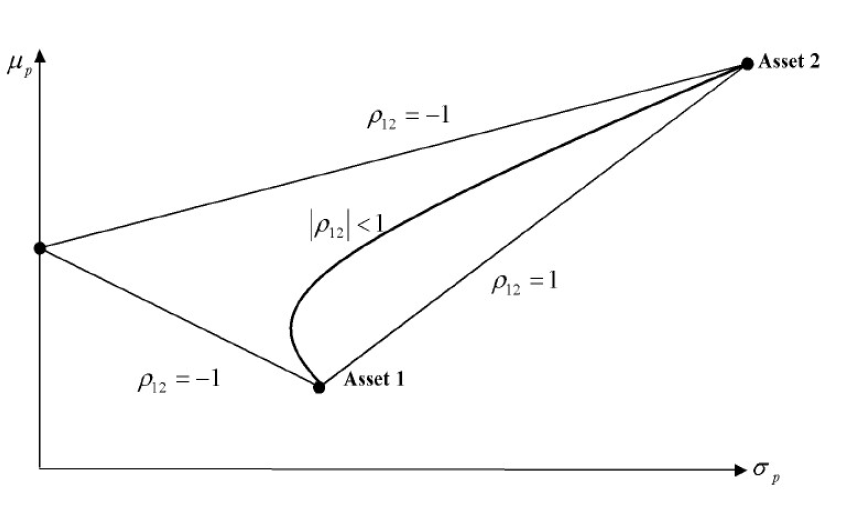
\includegraphics[width = 0.45\textwidth]{4_1.png}
\caption{$0\leq \alpha\leq 1$, when short selling is not allowed.}
\end{figure}
The feasible set will be extended by extending the corresponding line segments beyond the end points if short selling \textit{is} allowed.
\end{definition}
\subsubsection{Feasible Sets of Portfolio of Three or More Assets}
We construct the feasible sets intuitively by considering only the two-asset combination first, which gives rises to a finite set of hyperbolas and line segments. Next, we consider the combination of any two assets represented as two distinct points of these curves, which give rises to infinite number of hyperbolas and line segments. All the points on this infinite set will be inside the feasible set.

We will show that the feasible set of a portfolio with $n(>2)$ assets has the following property.
\begin{theorem}[Properties of Feasible Set]
\hfill\\\normalfont \begin{enumerate}
\item For any fixed $\mu\in\mathbb{R}$, $\exists \sigma>0$ such that $(\sigma,\mu)\in F$.
\item For each $(\sigma,\mu)\in F$, $(\sigma^\prime, \mu)\in F$ for all $\sigma^\prime>\sigma$.
\item For each pair of points $(\sigma, \mu)$ and $(\sigma^\prime, \mu^\prime)$ in the feasible set $F$, and for any $\lambda\in[0,1]$, the point $\lambda(\sigma,\mu)+(1-\lambda)(\sigma^\prime,\mu^\prime)$ lies in the set $F$. \\Equivalently, $F$ is a \textbf{convex set}.
\item For any fixed $\mu\in \mathbb{R}$, there exists $\sigma^\ast>0$ such that
\begin{enumerate}
\item $(\sigma^\ast,\mu)\in F$
\item if $(\sigma,\mu)\in F$, then $\sigma^\ast\leq \sigma$.
\end{enumerate}
We call this point $(\sigma^\ast, \mu)$ the \textbf{minimum-variance point} with mean $\mu$.
\end{enumerate}
\end{theorem}
\begin{definition}[Minimum-Variance Frontier]
\hfill\\\normalfont The theorem above suggests there is a minimum-variance point for any porfolio mean. The set of all minimum-variance points is called the \textbf{minimum-variance frontier}.
\end{definition}
It will be shown later that this minimum variance frontier is a \textbf{hyperbolic} curve.
\begin{definition}[Global Minimum Variance Point]
\hfill\\\normalfont The extreme left point on this frontier is called the \textbf{global minimum variance point}.
\end{definition}
\begin{definition}[Efficient Frontier]
\hfill\\\normalfont The minimum variance frontier \textit{above} the global minimum variance point is called the \textbf{efficient frontier}.
\end{definition}

\end{document}